\documentclass[hyperref={colorlinks}]{beamer}

\mode<presentation> {\usetheme{metropolis}}

\usepackage{graphicx} % Allows including images
\usepackage{booktabs} % Allows the use of \toprule, \midrule and \bottomrule in tables
\usepackage{algorithm}
\usepackage{algorithmic}
\usepackage{amsmath,amssymb,amsthm}
\usepackage[export]{adjustbox}

\newcommand{\set}[1]{\mathbb{#1}}
\newcommand{\trace}[1]{\mathrm{tr}\left(#1\right)}
\newcommand{\rank}[1]{\text{rank}\left(#1\right)}

\algsetup{
	linenosize=\footnotesize,
	linenodelimiter=.
}

%----------------------------------------------------------------------------------------
%	TITLE PAGE
%----------------------------------------------------------------------------------------

\title[QII Presentation]{PRIME: Novel Processing-in-memory Architecture for Neural Network Computation in ReRAM-based Main Memory} % The short title appears at the bottom of every slide, the full title is only on the title page
%\author{Ping Chi, Shuangchen Li, Cong Xu, Tao Zhang, Jishen Zhao, Yongpan Liu, Yu Wang and Yuan Xie}
\author{Presented by: Ravi Raju}
\institute[UW-Madison]{QII Presentation Spring 2018}
\date{March 23, 2018}

\begin{document}

\begin{frame}
	\titlepage
\end{frame}

\begin{frame}
	\frametitle{Overview}
	\tableofcontents
\end{frame}

%----------------------------------------------------------------------------------------
%	PRESENTATION SLIDES
%----------------------------------------------------------------------------------------

\section{Problem Statement and Solution}
\begin{frame}
	\frametitle{Problem Statement/Motivation}
	\begin{enumerate}
		\item Neural Networks 
		\begin{itemize}
			\item Popular for image/speech recognition application
			\item High Memory Bandwidth Requirement
		\end{itemize}
		\item Current Solutions
		\begin{itemize}
			\item DaDianNao - large on-chip eDRAM for high bandwith and data locality
			\item TrueNorth - SRAM crossbar memory for synapses
		\end{itemize}
		\item Both solutions suffer from latency of data movement
		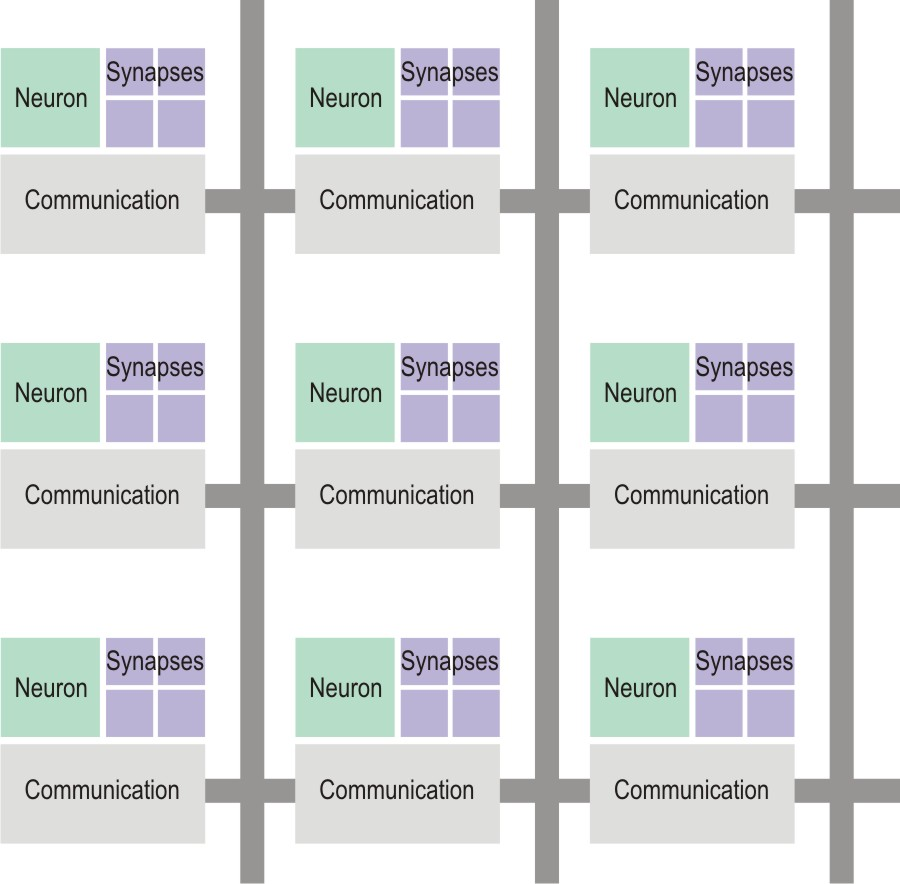
\includegraphics[scale=0.4, center]{ibm_sram_crossbar.jpg}
	\end{enumerate}
\end{frame}

\begin{frame}
	\frametitle{Proposed Solution: PRIME}
	\begin{enumerate}
		\item Processing in Memory is a natural solution
		\begin{itemize}
			\item Inspired by HMC
			\item Place compute units in memory to do NN computation
			\item Latency of In-memory data communication vs. DRAM memory access
		\end{itemize}
		\item PRIME
		\begin{itemize}
			\item ReRAM crossbar array solution
			\item Dynamically reconfigure between NN accerelation and memory
			\begin{enumerate}
				\item Architectural/circuit level support
				\item Software interface 
			\end{enumerate}
		\end{itemize}
		\item Targets large-scale MLP and CNN applications
		%\item Low area overhead
		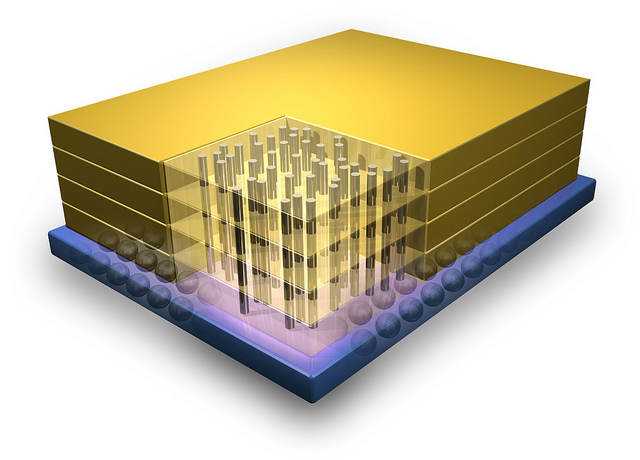
\includegraphics[scale=0.5,right]{hcm.jpg}
	\end{enumerate}
\end{frame}
\begin{frame}
	\frametitle{Key Idea: PRIME}
	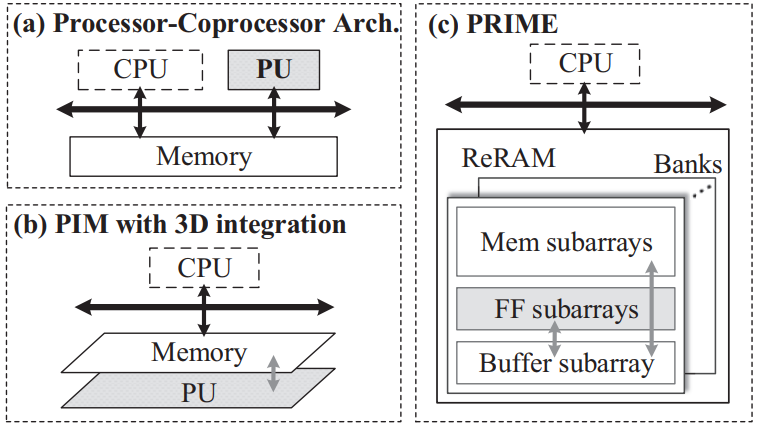
\includegraphics[scale=0.4]{keyIdea.png}
\end{frame}

\section{Background}
\begin{frame}
	\frametitle{What is ReRAM}
	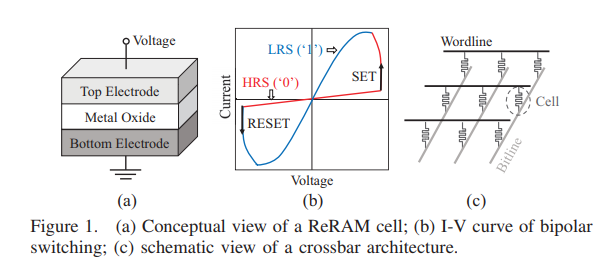
\includegraphics[scale=0.5]{reram.png}
\end{frame}

\begin{frame}
	\frametitle{What is a Neural Network}
	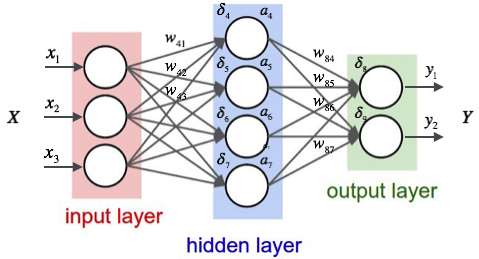
\includegraphics[scale=0.6]{nn.png}
\end{frame}

\begin{frame}
	\frametitle{ReRAM in relation to Neural Nets}
	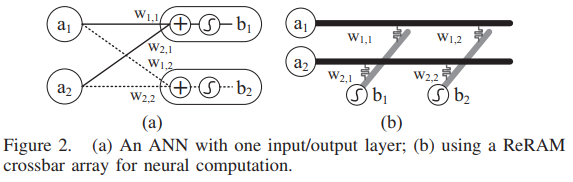
\includegraphics[scale=0.5]{reram_nn.png}
\end{frame}

\section{Architecture and System Design}
\begin{frame}
	\frametitle{High Level Overview of Architecture}
	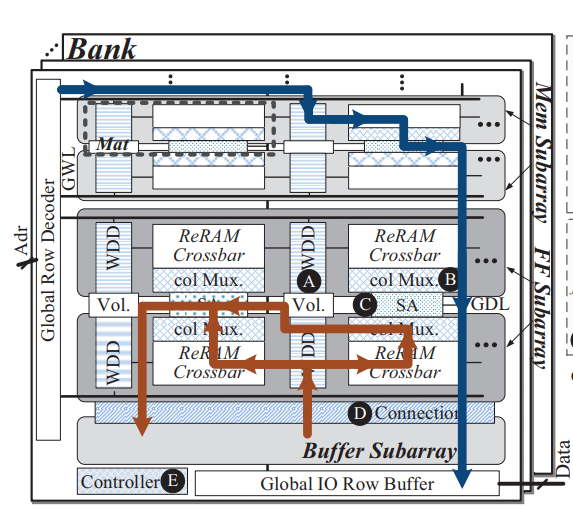
\includegraphics[scale=0.4, center]{prime_arch.png}
\end{frame}

\begin{frame}
	\frametitle{Choosing between NN Computation and Memory Mode}
	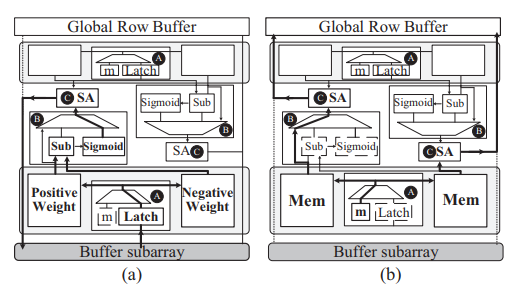
\includegraphics[scale=0.4, center]{NNvsMem.png}
\end{frame}

\begin{frame}
	\frametitle{MicroArchitecture of FF SubArray: Decoder}
	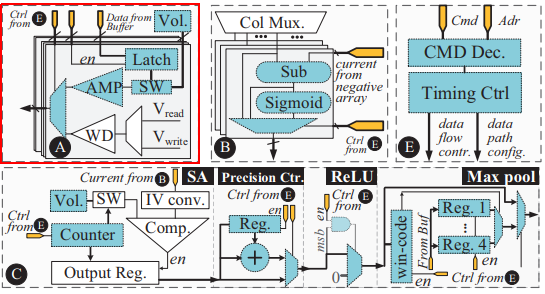
\includegraphics[scale=0.4, center]{decoder1.png}
\end{frame}

\begin{frame}
	\frametitle{MicroArchitecture of FF SubArray: Col Mux}
	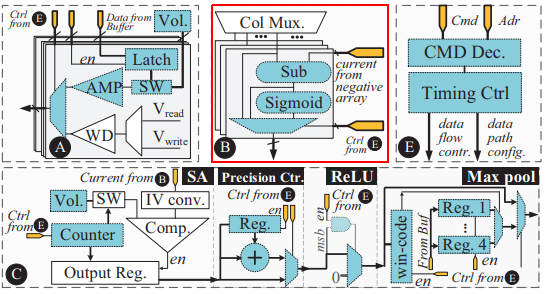
\includegraphics[scale=0.4, center]{col.png}
\end{frame}

\begin{frame}
	\frametitle{MicroArchitecture of FF SubArray: SA}
	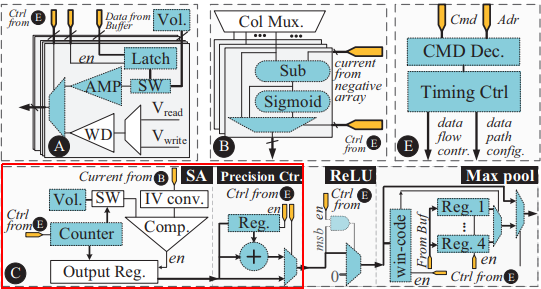
\includegraphics[scale=0.4, center]{SA.png}
\end{frame}

\begin{frame}
	\frametitle{Precision Issues}
	\begin{itemize}
		\item Input precision
		\item Weight precision
		\item Output precision
	\end{itemize}
	\begin{itemize}
		\item Multiple low-precision input signals
		\item Multiple cells to make one high precision weight
		\item Multiple phases for one computation
	\end{itemize}
\end{frame}

\begin{frame}
	\frametitle{System Level Design}
	\begin{itemize}
		\item Small-Scale NN: Replication
		\item Medium-Scale NN: Split-Merge
		\item Large-Scale NN: Inter-Bank Communication
	\end{itemize}
	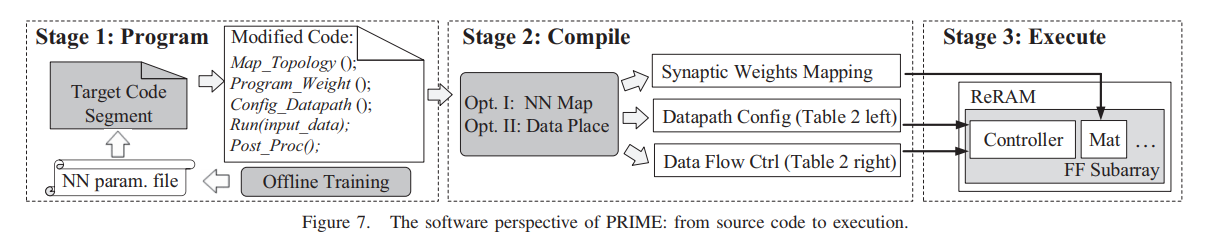
\includegraphics[scale=0.25]{system_level.png}	
\end{frame}

\section{Evaluations and Results}
\begin{frame}
	\frametitle{Experimental Setup}
	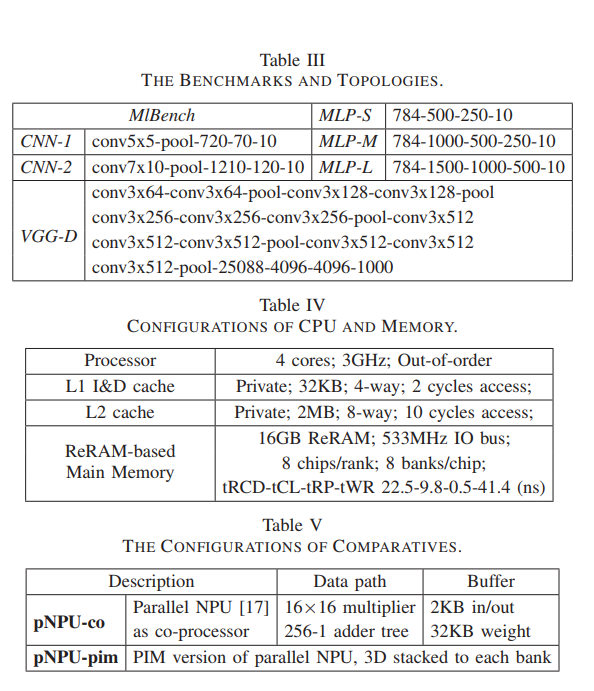
\includegraphics[scale=0.3, center]{ex_setup.png}	
\end{frame}

\begin{frame}
	\frametitle{Performance}
	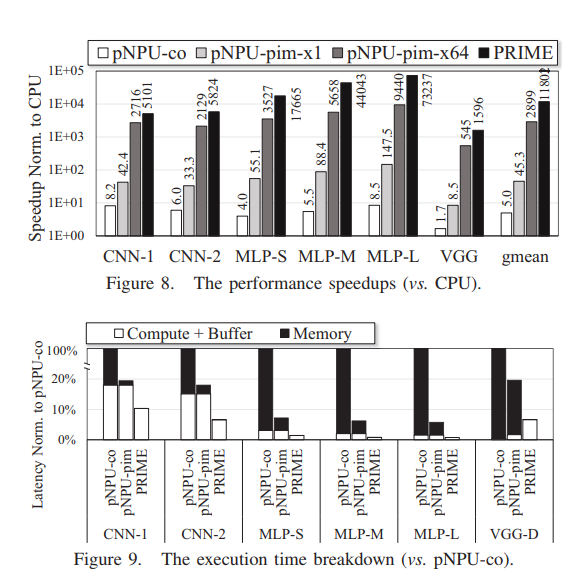
\includegraphics[scale=0.4, center]{performance.png}	
\end{frame}

\begin{frame}
	\frametitle{Energy}
	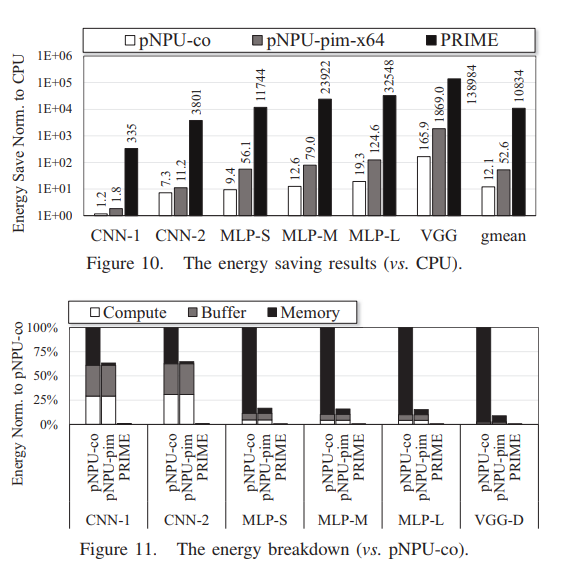
\includegraphics[scale=0.4, center]{energy.png}	
\end{frame}

\begin{frame}
	\frametitle{Area}
	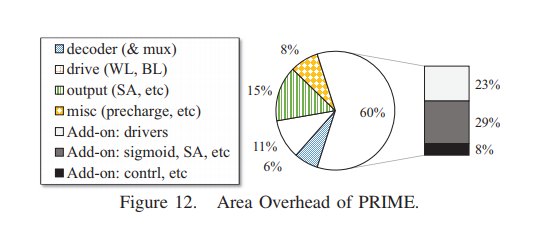
\includegraphics[scale=0.5, center]{area.png}	
\end{frame}

\section{Discussion}
\begin{frame}
	\frametitle{Critique}
	\begin{enumerate}
		\item PRIME only supports unsigned input vectors
		\item Dot-product computations in PRIME are lossy
		\begin{itemize}
			\item Precision of ADC does not always match precision of dot-product
		\end{itemize}
		\item Opportunity to exploit sparsity of NN for energy savings
		\begin{itemize}
			\item Introduce some logic into pipeline to check how many non-zero weights in crossbar
			\item If below some defined threshold, skip the computation
		\end{itemize}
	\end{enumerate}
\end{frame}
\begin{frame}
	\frametitle{Conclusion}
	\begin{itemize}
		\item PRIME is the solution to the data movement and high memory bandwidth problem
		\item Using ReRAM crossbar accerlerates NN computation
		\item Circuit/microarchitectural changes as well as software interface enables wide spectrum of NN applications
		\item Very little area overhead and extra processing elements
	\end{itemize}
\end{frame}
%------------------------------------------------

\begin{frame}
	\frametitle{References}
	\footnotesize{
		\begin{thebibliography}{9} % Beamer does not support BibTeX so references must be inserted manually as below
			\bibitem[Chi, 2016]{chi2016}
			P. Chi, et al. (2016, Sept. 4).
			\emph{PRIME: A Novel Processing-in-Memory Architecture for Neural Network Computation in ReRAM-Based Main Memory} [Online].
			Available: \url{http://ieeexplore.ieee.org/document/7551380/citations?tabFilter=papers}
			\bibitem[Shafiee, 2016]{shafiee2016}
			A. Shafiee, et al. (2016, Aug. 25).
			\emph{ISAAC: A Convolutional Neural Network Accelerator with In-Situ Analog Arithmetic in Crossbars} [Online].
			Available: \url{http://ieeexplore.ieee.org/document/7551379/}
		\end{thebibliography}
	}
\end{frame}
%------------------------------------------------

\begin{frame}
	\Huge{\centerline{Thank you and Questions}}
\end{frame}

\begin{frame}
	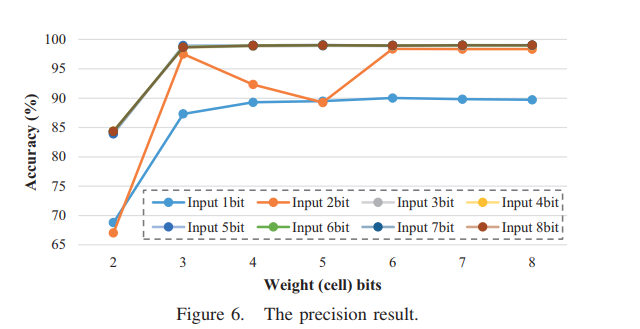
\includegraphics[scale=0.4]{precision_graph.png}
\end{frame}



\end{document} 